\documentclass[11pt]{article}

\usepackage[margin=1in]{geometry}
\usepackage{amsmath,amssymb}
\usepackage{booktabs}
\usepackage{hyperref}
\usepackage{pgfplots}
\pgfplotsset{compat=1.18}

\title{Distance-Banded Low-Dimensional Attention: Initial Notes}
\author{}
\date{\today}

\begin{document}
\maketitle

\section{Motivation}

Standard causal self-attention computes pairwise scores
\begin{equation}
    s_{ij} = q_i^\top k_j,
    \qquad j \leq i,
\end{equation}
where all previous tokens interact through the same head dimension. The motivating hypothesis is that nearby tokens often require high-resolution token-level matching, while far-away tokens may only need a lower-dimensional interaction space. If true, attention could spend more representational and computational budget on local context and less on distant context.

The proposed modification is to make the attention score distance-dependent:
\begin{equation}
    s_{ij} = (P_{b(i-j)} q_i)^\top (P_{b(i-j)} k_j),
\end{equation}
where $b(i-j)$ maps the causal distance $i-j$ to a distance band, and $P_b$ projects into a band-specific lower-dimensional subspace. In the pilot experiments, the bands were
\begin{equation}
    [0,128] \mapsto 64,\qquad
    [129,512] \mapsto 32,\qquad
    [513,\infty) \mapsto 16,
\end{equation}
where the numbers on the right are per-head query/key dimensions. A later aggressive-compression run changed the medium and far dimensions to 16 and 8.

\section{Variants Tested}

We tested three attention modes:

\paragraph{Baseline.}
The baseline uses standard causal attention:
\begin{equation}
    s_{ij} = q_i^\top k_j.
\end{equation}
In the current implementation, this uses PyTorch scaled dot-product attention and therefore benefits from FlashAttention.

\paragraph{Distance prefix.}
This mode uses a single shared query/key projection as in the baseline, but each distance band scores only a prefix of the head vector:
\begin{equation}
    s_{ij}^{(b)} =
    q_{i,1:d_b}^\top k_{j,1:d_b}.
\end{equation}
This is the simplest version of the idea: far-away interactions use fewer coordinates, but the coordinates are shared with the near-token representation.

\paragraph{Distance per band.}
This mode gives each band its own learned query/key projections:
\begin{equation}
    q_i^{(b)} = W_Q^{(b)} x_i,\qquad
    k_j^{(b)} = W_K^{(b)} x_j,\qquad
    s_{ij}^{(b)} = \left(q_i^{(b)}\right)^\top k_j^{(b)}.
\end{equation}
This allows the model to learn separate matching spaces for near, medium, and far context.

\section{Benchmark Setup}

The initial language-modeling test used the Parameter Golf-style FineWeb objective with the small GPT configuration currently in the repository:

\begin{itemize}
    \item sequence length: 1024
    \item model width: 512
    \item layers: 9
    \item attention heads: 8
    \item KV heads: 4
    \item training tokens per step: 524,288
    \item iterations: 800
    \item validation cadence: every 200 steps
    \item default distance bands: \texttt{128:64,512:32,inf:16}
    \item aggressive distance bands: \texttt{128:64,512:16,inf:8}
\end{itemize}

The custom distance modes currently use a chunked and checkpointed dense implementation to avoid out-of-memory errors. This makes them runnable for quality experiments, but they do not yet realize the intended speedup. The baseline uses FlashAttention, while the custom modes do not.

\section{Initial Results}

\begin{table}[h]
\centering
\small
\begin{tabular}{llrrrr}
\toprule
Mode & Bands & Final train loss & Val loss & Val BPB & Step time (ms) \\
\midrule
Baseline & -- & 2.3065 & 2.3308 & 1.3804 & 864.35 \\
Distance per band & 64/32/16 & 2.3023 & 2.3290 & 1.3794 & 3137.88 \\
Distance prefix & 64/32/16 & 2.3134 & 2.3413 & 1.3867 & 2983.04 \\
Distance per band & 64/16/8 & 2.3112 & 2.3394 & 1.3855 & 3176.41 \\
\bottomrule
\end{tabular}
\caption{Single-seed 800-step Parameter Golf pilot runs. Lower validation loss and BPB are better.}
\end{table}

\begin{figure}[h]
\centering
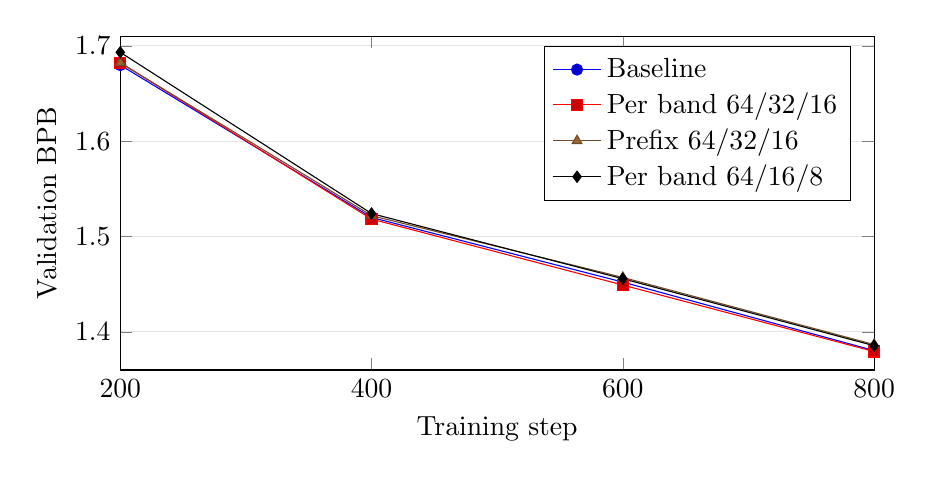
\begin{tikzpicture}
\begin{axis}[
    width=0.92\linewidth,
    height=0.48\linewidth,
    xlabel={Training step},
    ylabel={Validation BPB},
    xmin=200, xmax=800,
    ymin=1.36, ymax=1.71,
    xtick={200,400,600,800},
    ymajorgrids=true,
    grid style={gray!20},
    legend pos=north east,
    legend cell align={left},
]
\addplot+[mark=*] coordinates {
    (200,1.6798) (400,1.5200) (600,1.4522) (800,1.3804)
};
\addlegendentry{Baseline}
\addplot+[mark=square*] coordinates {
    (200,1.6823) (400,1.5183) (600,1.4491) (800,1.3794)
};
\addlegendentry{Per band 64/32/16}
\addplot+[mark=triangle*] coordinates {
    (200,1.6822) (400,1.5219) (600,1.4571) (800,1.3867)
};
\addlegendentry{Prefix 64/32/16}
\addplot+[mark=diamond*] coordinates {
    (200,1.6932) (400,1.5241) (600,1.4557) (800,1.3855)
};
\addlegendentry{Per band 64/16/8}
\end{axis}
\end{tikzpicture}
\caption{Validation BPB trajectories after the initial step-0 evaluation. The curves are close; the final differences are easier to interpret as step-equivalent lags.}
\end{figure}

The main observation is that \texttt{distance\_per\_band} essentially matched the baseline in validation quality in this short run:
\begin{equation}
    \Delta \mathrm{BPB}
    =
    1.3794 - 1.3804
    =
    -0.0010.
\end{equation}
This difference is small enough that it should be treated as noise until tested across more seeds, but it is encouraging: the lower-dimensional far-context interaction did not obviously hurt the model.

The \texttt{distance\_prefix} variant was worse:
\begin{equation}
    \Delta \mathrm{BPB}
    =
    1.3867 - 1.3804
    =
    +0.0063.
\end{equation}
This suggests that simply truncating a shared query/key vector may be too restrictive. The model appears to benefit from learning separate distance-specific matching spaces.

The more aggressive \texttt{distance\_per\_band} run used \texttt{128:64,512:16,inf:8}. It landed between the mild per-band run and the prefix run:
\begin{equation}
    1.3855 - 1.3804 = +0.0051
\end{equation}
BPB worse than baseline, and
\begin{equation}
    1.3855 - 1.3794 = +0.0061
\end{equation}
BPB worse than the \texttt{64/32/16} per-band setting. This suggests that the far-context dimensions can likely be reduced, but the \texttt{16/8} medium/far setting may be too aggressive at this model scale and training horizon.

\subsection{Step-Equivalent Interpretation}

The raw BPB differences are small, so a useful scale is to compare them against the slope of the baseline learning curve. From step 600 to step 800, the baseline improves from 1.4522 BPB to 1.3804 BPB:
\begin{equation}
    \frac{1.4522 - 1.3804}{200}
    \approx
    0.000359
    \quad \mathrm{BPB/step}.
\end{equation}
Using this final-segment slope, each method's final BPB gap can be converted into an approximate number of baseline training steps.

\begin{table}[h]
\centering
\begin{tabular}{lrr}
\toprule
Mode & Final BPB gap vs baseline & Step-equivalent lag \\
\midrule
Distance per band 64/32/16 & $-0.0010$ & $\approx$ 3 steps ahead \\
Distance per band 64/16/8 & $+0.0051$ & $\approx$ 14 steps behind \\
Distance prefix 64/32/16 & $+0.0063$ & $\approx$ 18 steps behind \\
\bottomrule
\end{tabular}
\caption{Approximate final gaps measured in units of late-stage baseline training progress. Negative BPB gap means better than baseline.}
\end{table}

This framing suggests that the mild per-band model is effectively tied with baseline at this resolution, while the aggressive per-band and prefix variants lag by only a small fraction of the 800-step run. This is not a substitute for multi-seed statistics, but it gives the final differences a more intuitive scale.

\section{Interpretation}

The initial result supports a narrow but useful claim: distance-dependent query/key dimensionality can preserve short-run language-model quality, at least when implemented with learned per-band projections. It does not yet support a speed claim, because the current custom implementation is much slower than the FlashAttention baseline:
\begin{equation}
    \frac{3137.88}{864.35} \approx 3.63.
\end{equation}

Thus the current conclusion is:
\begin{quote}
The architectural idea is not obviously quality-destructive, and the per-band projection structure looks more promising than prefix truncation. However, a real efficiency result requires a fused or genuinely banded attention implementation that avoids materializing dense score matrices.
\end{quote}

\section{Next Experiments}

Natural next tests are:

\begin{enumerate}
    \item Run more seeds at the same 800-step setting to estimate noise.
    \item Sweep intermediate compression settings, e.g. \texttt{128:64,512:24,inf:12}.
    \item Compare parameter-matched versions, since \texttt{distance\_per\_band} changes the query/key parameterization.
    \item Implement a fused/windowed kernel or block-sparse attention path so the method can be tested for actual speed and memory improvements.
\end{enumerate}

\end{document}
